\iffalse
\documentclass[12pt]{article}
\usepackage{graphicx}
\usepackage[none]{hyphenat}
\usepackage{graphicx}
\usepackage{listings}
\usepackage[english]{babel}
\usepackage{graphicx}
\usepackage{caption} 
\usepackage{booktabs}
\usepackage{array}
\usepackage{amssymb} % for \because
\usepackage{amsmath}   % for having text in math mode
\usepackage{extarrows} % for Row operations arrows
\usepackage{listings}
\lstset{
  frame=single,
  breaklines=true
}
\usepackage{hyperref}
  
%Following 2 lines were added to remove the blank page at the beginning
\usepackage{atbegshi}% http://ctan.org/pkg/atbegshi
\AtBeginDocument{\AtBeginShipoutNext{\AtBeginShipoutDiscard}}
\usepackage{gensymb}


%New macro definitions
\newcommand{\mydet}[1]{\ensuremath{\begin{vmatrix}#1\end{vmatrix}}}
\providecommand{\brak}[1]{\ensuremath{\left(#1\right)}}
\providecommand{\sbrak}[1]{\ensuremath{{}\left[#1\right]}}
\providecommand{\norm}[1]{\left\lVert#1\right\rVert}
\providecommand{\abs}[1]{\left\vert#1\right\vert}
\newcommand{\solution}{\noindent \textbf{Solution: }}
\newcommand{\myvec}[1]{\ensuremath{\begin{pmatrix}#1\end{pmatrix}}}
\let\vec\mathbf


\begin{document}

\begin{center}
\title{\textbf{Chords}}
\date{\vspace{-5ex}} %Not to print date automatically
\maketitle
\end{center}
\setcounter{page}{1}

\section{12$^{th}$ Maths - Chapter 8}
This is Problem-13 from Exercise 8.1 
\begin{enumerate}

\solution 
\item 
	\fi
	The given equation of the curve can be rearranged as
\begin{align}
	y^2-4x &= 0 \\
        \label{eq:chapters/12/8/1/13/Eq1}
	\implies \vec{x}^\top\myvec{0 & 0 \\ 0 & 1}\vec{x} + 2\myvec{-2 & 0}\vec{x}+0 &= 0 
\end{align}
The above equation can be equated to the generic equation of conic sections
\begin{align}
	\label{eq:chapters/12/8/1/13/Eq2}
	g\brak{\vec{x}} = \vec{x}^T\vec{V}\vec{x} + 2\vec{u}^T\vec{x} + f = 0 
\end{align}
Comparing coefficients of both equations \eqref{eq:chapters/12/8/1/13/Eq1} and \eqref{eq:chapters/12/8/1/13/Eq2} 
\begin{align}
	\vec{V} &= \myvec{ 0 & 0 \\ 0 & 1} \\
	\vec{u} &= \myvec{-2 \\ 0} \\
	f &= 0
\end{align}
For the given line $y=3$, the parameters are
\begin{align}
	\vec{h} = \myvec{0 \\ 3} , \vec{m} = \myvec{1 \\ 0 }
\end{align}
To calculate the point of contact of line with the conic, we use
\begin{align}
	\label{eq:chapters/12/8/1/13/Eq3}
	\mu^2\vec{m}^\top\vec{V}\vec{m}+2\mu\vec{m}^\top\brak{\vec{V}\vec{h}+\vec{u}}+g\brak{\vec{h}}= 0 
\end{align}
\begin{multline}
	g\brak{\vec{h}}=\myvec{0 & 3}\myvec{0 & 0 \\ 0 & 1}\myvec{0 \\3} \\
	+ 2\myvec{-2 & 0}\myvec{0 \\ 3} + 0 \\
	 \implies g\brak{\vec{h}} = \myvec{0 & 3}\myvec{0 \\3} + 2\myvec{0} \\ 
	 \implies g\brak{\vec{h}} = 9 
\end{multline}
\begin{multline}
	\eqref{eq:chapters/12/8/1/13/Eq3} \implies \mu^2\myvec{1 & 0}\myvec{0 & 0 \\ 0 & 1}\myvec{1 \\ 0} \\
	 + 2\mu\myvec{1 & 0}\brak{\myvec{0 & 0 \\ 0 & 1}\myvec{0 \\3}+\myvec{-2 \\ 0}} + 9 = 0 \\
	\implies \mu^2\brak{0}+2\mu\myvec{1 & 0}\myvec{-2 \\3} + 9 = 0 \\
	\implies -4\mu + 9 = 0  \\
	\implies \mu  = \frac{9}{4} 
\end{multline}
The point of contact is given as
\begin{align}
	\vec{a}_0 = \myvec{\frac{9}{4}  \\[1pt] \\ 3}
\end{align}
The desired area of the region is given as
\begin{align}
	\int_{0}^{3} \ \frac{y^2}{4} \,dy &= \frac{1}{12}\sbrak{y^3}_{0}^{3} \\
	&= \frac{1}{12}\brak{27-0} \\
	&= \frac{9}{4} \text{ sq.units}
\end{align}
The relevant diagram is shown in Figure \ref{fig:chapters/12/8/1/13/Fig1}
\begin{figure}[!h]
	\begin{center}
		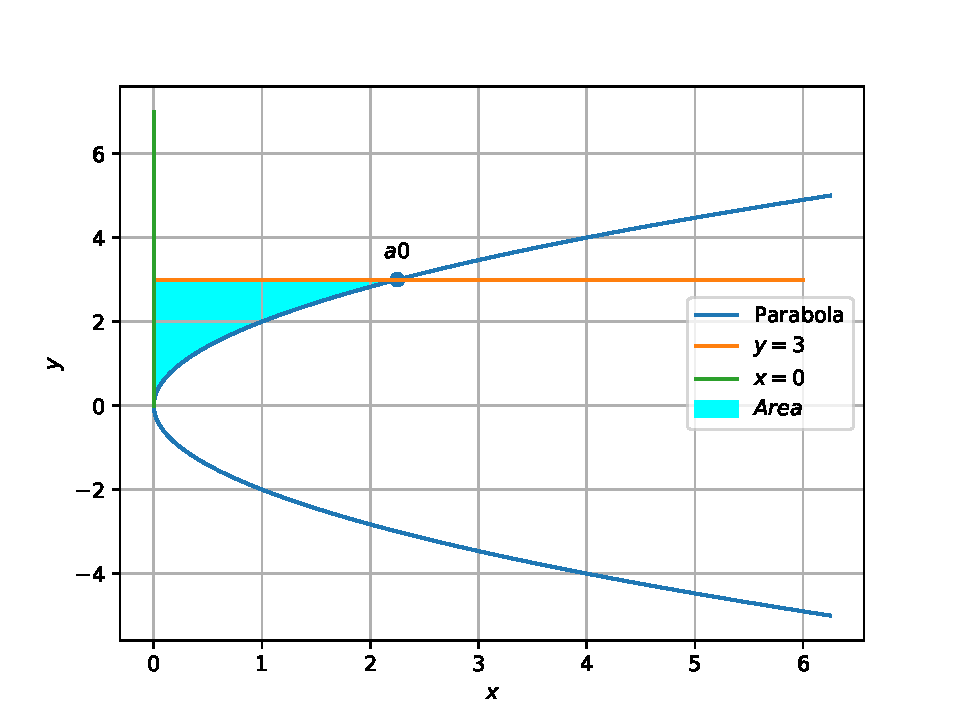
\includegraphics[width=\columnwidth]{chapters/12/8/1/13/figs/problem13.pdf}
	\end{center}
\caption{}
\label{fig:chapters/12/8/1/13/Fig1}
\end{figure}
